\documentclass[../PHYS306Notes.tex]{subfiles}

\begin{document}
\subsection{Worksheet - Rotating Coordinate Systems}
\begin{center}
    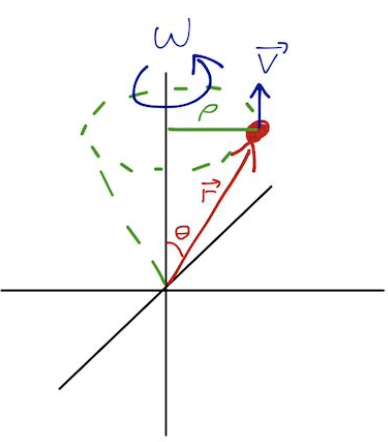
\includegraphics[scale=0.75]{Lecture-15/w15-img1.png}
\end{center}
\begin{p}
What is the time rate of change, $\od{\v{r}}{t} = \v{v}$ of a vector $\v{r}$ to a point in a body that is rotating about an axis $O$ with angular velocity $\omega$?
\end{p}
\begin{s}
We define the rotation vector:
\[\bm{\omega} = \omega\hat{\v{u}}\]
Where $\hat{\v{u}}$ points along the rotation axis (the sign is determined by the RHR). Geometry tells us that the distance from the rotation axis $\rho$ is given by:
\[\rho = r\sin\theta\]
Hence the velocity of this point is given by:
\[v = \rho\omega = r\sin\theta\omega\]
Generalizing this to the vector form, we have:
\[\v{v} = \bm{\omega} \times \v{r} = \dot{\v{r}}\]
\end{s}

\begin{p}
Consider a body rotating in a reference frame that is itself rotating with respect to a fixed reference frame. Show that angular velocities add just like linear velocities.
\end{p}
\begin{s}
This is a consequence of the linearity of the cross product. Suppose we have:
\[\v{v}_{31} = \bm{\omega}_{31}\times \v{r} = \v{v}_{32} + \v{v}_{21} = \bm{\omega}_{32}\times \v{r} + \bm{\omega}_{21}\times \v{r} = (\bm{\omega}_{32} + \bm{\omega}_{21})\times \v{r}\]
Hence:
\[\bm{\omega}_{31} = \bm{\omega}_{32} + \bm{\omega}_{21}\]
So we can see that we can add angular velocities just like linear velocities.
\end{s}

\begin{p}
Consider a vector $\v{Q}$, which may be a position, velocity, or force vector. Show that the time rate of change of $\v{Q}$, $\od{\v{Q}}{t}$ in a fixed frame of reference $S_0$ is related to $\od{\v{Q}}{t}$ in a rotating frame of reference $S$ by:
\[\left(\dod{\v{Q}}{t}\right)_{S_0} = \left(\dod{\v{Q}}{t}\right)_{S} + \v{\Omega} \times \v{Q}\]
\end{p}
\begin{s}
\begin{center}
    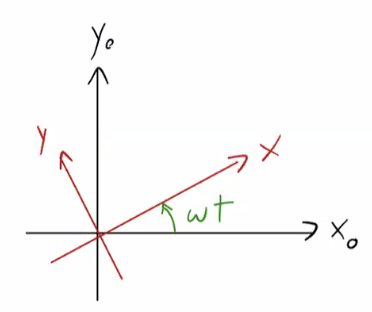
\includegraphics[scale=0.75]{Lecture-15/w15-img2.png}
\end{center}
We express the unit vectors in the rotating frame by transforming the unit vectors in the fixed frame:
\[\xhat = \xhat_0\cos\omega t + \yhat_0\sin\omega t\]
\[\yhat = \yhat_0\cos\omega t - \xhat_0\sin\omega t\]
So expressing an arbitrary vector $\v{Q}$ in the rotating frame, we have:
\[\v{Q} = Q_x\xhat + Q_y\yhat + Q_z\zhat\]
Now expressing this in terms of the unit vectors in the stationary frame, we have:
\[\v{Q} = (Q_x\cos\omega t - Q_y\sin\omega t)\xhat_0 + (Q_x\sin\omega t + Q_y\cos\omega t)\yhat_0 + Q_z\zhat_0\]
We pick $\zhat$ to be the rotation axis, so $\zhat = \zhat_0$ by our choice of coordinate system. Looking at the rate of change w.r.t the lab frame, we have:
\[\left(\dod{\v{Q}}{t}\right)_{S_0} = \left(-\omega Q_x\sin\omega t - \omega Q_y\cos\omega t\right)\xhat_0 + \left(\omega Q_x\cos\omega t - \omega Q_y \sin \omega t\right)\yhat_0 \]
Where the unit vectors do not have time dependence, only the $\cos\omega t$ and $\sin\omega t$ terms do. Looking at this expression, we can see that this can be written as the expression:
\[\left(\dod{\v{Q}}{t}\right)_{S_0} = \omega(\zhat_0 \times \v{Q}) = \bm{\omega} \times \v{Q}\]
Now, we take the derivative in the rotating frame:
\[\left(\dod{\v{Q}}{t}\right)_{S} = \dot{Q}_x\xhat + \dot{Q}_y \yhat + \dot{Q}_z \zhat\]
Now, we consider what is $\left(\od{Q}{t}\right)_{S_0, x}$. By the chain rule:
\[\left(\od{Q}{t}\right)_{S_0, x} = \dod{}{t}\left(Q_x\cos\omega t - Q_y\sin\omega t\right)\xhat_0\]
\[\left(\od{Q}{t}\right)_{S_0, x} = \left[\dot{Q}_x\cos\omega t - \dot{Q}_y\sin\omega t) + (-\omega Q_x\sin\omega t - \omega Q_y\cos\omega t)\right]\xhat_0\]
Doing the same for the $x$ and $y$ components, we get the simple formula:
\[\left(\dod{\v{Q}}{t}\right)_{S_0} = \left(\dod{\v{Q}}{t}\right)_{S} + \bm{\omega}\times\v{Q}\]
\end{s}

\begin{p}
Now find the acceleration in a fixed frame of reference, and thus write the modified Newton’s law for a constantly rotating frame of reference, as we’d experience on the earth for example. 
\end{p}
\begin{s}
The goal is to find the second derivative of the position vector in the $S$ (rotating) frame. First calculating $\left(\od[2]{\v{r}}{t}\right)_{S_0}$, we have:
\[\left(\dod[2]{\v{r}}{t}\right)_{S_0} = \left(\dod{}{t}\right)_{S_0}\left(\dod{\v{r}}{t}\right)_{S_0}\]
So applying the result from above twice, we have:
\[\left(\dod[2]{\v{r}}{t}\right)_{S_0} = \left(\dod{}{t}\right)_{S_0}\left(\left(\dod{\v{r}}{t}\right)_S + \bm{\Omega} \times \v{r}\right)\]
\[\left(\dod[2]{\v{r}}{t}\right)_{S_0} = \left(\dod{}{t}\right)_{S}\left(\left(\dod{\v{r}}{t}\right)_S + \bm{\Omega} \times \v{r}\right) + \bm{\Omega}\times \left(\left(\dod{\v{r}}{t}\right)_S + \bm{\Omega} \times \v{r}\right)\]
We now simplify this expression. Henceforth, we will use the dot notation to refer to a derivative in $S$. \[\left(\dod[2]{\v{r}}{t}\right)_{S_0} =
\ddot{\v{r}} + \dot{\bm{\Omega}}\times \v{r} + \bm{\Omega} \times \dot{\v{r}} + \bm{\Omega} \times \dot{\v{r}} + \bm{\Omega} \times (\bm{\Omega} \times \v{r})\]
Multiplying both sides by $m$, and simplifying using the antisymmetry of the cross product ($\v{a} \times \v{b} = -\v{b} \times \v{a}$) have:
\[m\left(\dod[2]{\v{r}}{t}\right)_{S_0} = \v{F} = 
m\ddot{\v{r}} - 2m\dot{\v{r}}\times\bm{\Omega} - m(\dot{\v{r}}\times \dot{\bm{\Omega}}) - m(\bm{\Omega} \times \v{r}) \times \bm{\Omega}\] 
Where we use the identity that the LHS is just the total force on the system by Newton's second law. Rearranging this, we have:
\[m\ddot{\v{r}} = \v{F} + 2m\dot{\v{r}}\times \bm{\Omega} + m(\bm{\Omega} \times \v{r})\times \bm{\Omega} + m(\v{r} \times \dot{\bm{\Omega}})\]
Where the first term is the sum of the (real) forces on the system, the second term is the coriolois force, the third term is the centrifugal force, and the fourth term (which is nonzero only if the angular velocity is changing in time) is the Euler force. We may write this as:
\[m\ddot{\v{r}} = \v{F} + \v{F}_{cor} + \v{F}_{cent} + \v{F}_{euler}\]
We note that we can also derive this using the Lagrangian approach! If we write the Lagrangian with the correct velocity, i.e.:
\[\LL = \frac{m}{2}\left|\left(\dod{r}{t}\right)_{S_0}\right|^2 - U(\v{r})\]
Then we will find that we recover the same result.

\end{s}
\end{document}